\chapter{Methodologie}
Dit hoofdstuk beschrijft hoe we de eerder beschreven theoretische componenten samen hebben gevoegd tot een automatische generator van beschrijvingen. Een eerste sectie handelt over een bestaande implementatie, waarop ons systeem is gebaseerd. De volgende twee secties handelen over mogelijkheden om extra semantische informatie toe te voegen: LDA en de Flickr30k Entities, gevolgd door een uitgebreide beschrijving hoe we deze informatie juist toevoegen. Een volgende sectie gaat over onze implementatie van het eerder vernoemde gLSTM netwerk zoals voorgesteld door Jia \todo{reference?}. De laatste sectie beschrijft hoe wij een normalisatie hebben toegevoegd aan de beam search om zinnen te maken (zoals voorgesteld door Jia \todo{ref}).

\section{Startpunt Karpathy} \todo{Betere titel}
Het startpunt van onze implementatie is de code aangereikt door A. Karpathy op zijn github pagina\footnote{https://github.com/karpathy/neuraltalk}. Die bevat een implementatie van het recurrente neurale netwerk beschreven in \todo{reference naar karpathy}, alsook een implementatie die gebaseerd is op \todo{reference vinyals}. Vertrekkende van deze code hebben wij een aantal extensies ge\"implementeerd.
\subsection{Recurrent Neuraal Netwerk}
Een eerste implementatie waarvan we zijn vertrokken is beschreven in Karpathy\todo{ref!}. Hij beschrijft een systeem dat op basis van een afbeelding een beschrijvende zin genereert. Dit gebeurt in twee stappen. Eerst wordt de afbeelding door middel van een CNN omgezet naar een vector representatie. Deze vector dient vervolgens als input voor een recurrent neuraal netwerk dat een grammaticaal correcte beschrijving genereert.

\paragraph{Afbeeldingsrepresentatie}
Het dataformaat van een afbeelding (2D matrix met een RGB waarde voor elke pixel) is onpraktisch om te gebruiken in neurale netwerken, aangezien die algemeen gesproken gevectoriseerde input vragen. Er is dus nood aan een vectorrepresentatie van de gebruikte afbeeldingen. De meeste bestudeerde algoritmes maken hiervoor gebruik van een convolutioneel neuraal netwerk (CNN).

Het CNN dat momenteel het beste presteert is VGGNet, zoals beschreven in \todo{ref VGGNet}. Dit netwerk maakt gebruik van 16 layers, wat ervoor zorgt dat er een extreem diep netwerk is, wat complexere verbanden kan leren. De lagen bestaan uit groepen van convolutionele layers afgewisseld met max-pool layers. Bij max-pooling wordt de afbeelding gesplitst in een aantal regio's. De maxima van alle regio's vormen dan een down-sampled weergave van de input. Figuur \ref{fig:maxpool} \todo{Reference: afbeelding van wikimedia} illustreert het principe van max-pooling met een filtergrootte van 2x2 en een stapgrootte van 2, wat VGGNet ook gebruikt.

\begin{figure}[tb]
    \centering
    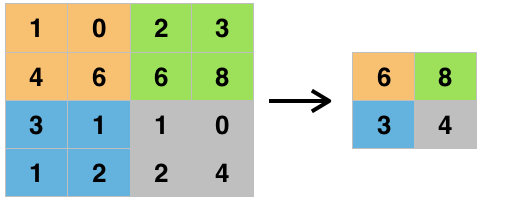
\includegraphics[width=0.6\linewidth]{Images/maxpool.png}
    \caption{Max pooling met 2x2 filter en stapgrootte 2}
    \label{fig:maxpool}
\end{figure}

De laatste layers van het netwerk zijn standaard (volledig verbonden) layers, gevolgd door een softmax layer om de output van het netwerk te normaliseren. Figuur \ref{fig:alexvgg} toont een vereenvoudigde weergave van de architectuur van VGGNet, in vergelijking met het vroeger zeer populaire AlexNet \todo{reference naar paper voor afbeelding, en naar alexnet, vggnet}.

\begin{figure}[tb]
    \centering
    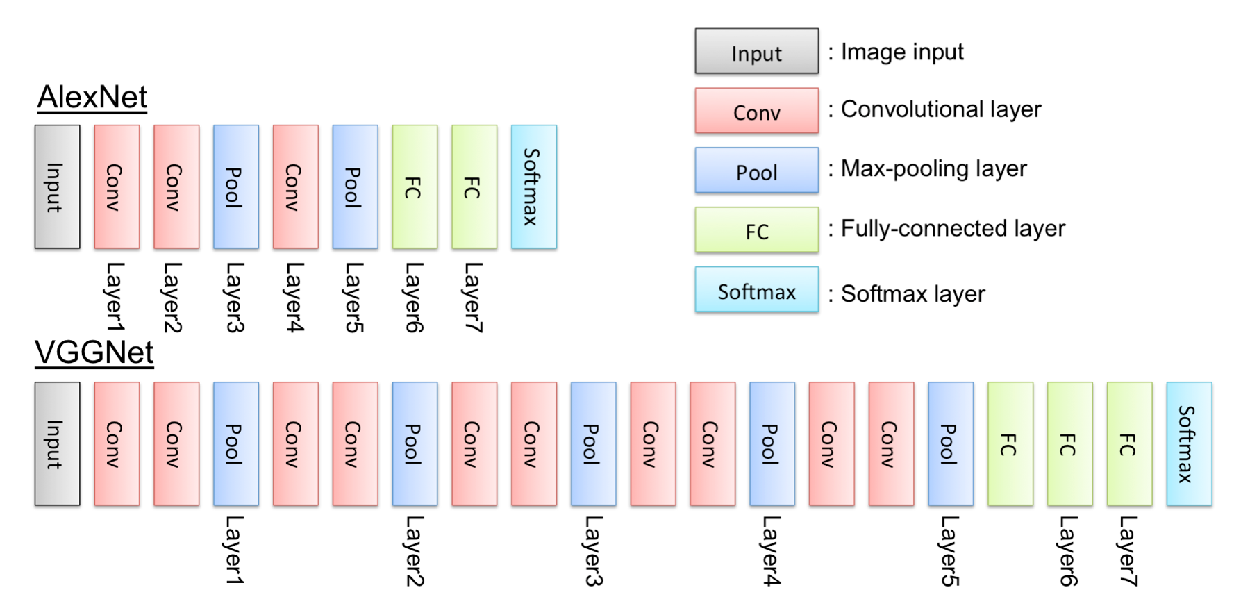
\includegraphics[width=\linewidth]{Images/alex_vgg.eps}
    \caption{Vergelijking van de architectuur van AlexNet en VGGNet}
    \label{fig:alexvgg}
\end{figure}


De representatie die wordt gebruik door Karpathy is het resultaat van het netwerk voor de softmax layer wordt toegepast. Dit leidt tot een 4096-dimensionele vector, waarbij elke dimensie kan worden gezien als een bepaald concept dat al dan niet aanwezig is in de afbeelding. Deze dimensionaliteit is dezelfde voor alle afbeeldingen, onafhankelijk van de grootte van de input. Dit komt door een herschaling alvorens de afbeeldingsvector te berekenen.

VGGNet is momenteel het best presterende CNN voor afbeeldingsrepresentatie. Wij gebruiken in ons systeem dan ook de afbeeldingsvectors die berekend zijn met VGGNet. De gebruikte implementatie komt van Caffe \todo{Reference Caffe}.

\paragraph{Van afbeelding naar beschrijving}
De berekende vector representatie van de afbeelding dient als input voor een recurrent neuraal netwerk. Tijdens de training van het netwerk wordt op basis van de afbeelding, in combinatie met een speciale startvector die het begin van een zin aangeeft, het eerste woord voorspeld. Daarna wordt op basis van het eerste woord van de zin een voorspelling gemaakt voor het tweede woord. Dit proces herhaalt zich tot het einde van de zin bereikt is. Terugpropagatie op basis van stochastic gradient descent zorgt voor de juiste wijzigingen aan de gewichten van het netwerk. Een eenvoudige weergave van hoe het RNN een beschrijving genereert is te zien op figuur \ref{fig:rnntraining}.

\begin{figure}[tb]
    \centering
    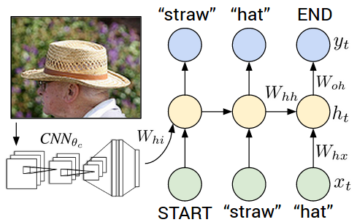
\includegraphics[width=0.5\linewidth]{Images/karpathy.PNG}
    \caption{Generatie van caption met recurrent neuraal netwerk}
\label{fig:rnntraining}
\end{figure}

Het trainen van het RNN gebeurt op basis van de Flickr30k dataset. Er worden random afbeeldingen met 1 van de 5 bijhorende beschrijvingen aan het netwerk gegeven. De eerder vermeldde terugpropagatie zorgt voor de juiste aanpassing aan de gewichten. Wanneer de trainingsset volledig is doorlopen vindt een evaluatie plaats. De perplexity berekend op de resultaten voor de validatieset geeft snel aan of het netwerk nog bijleert of niet. Wanner we merken dat er geen daling meer is in perplexity zetten we het trainingsproces stop.

De code van Karpathy voorziet ook de optie om gebruik te maken van ReLu encoders, deze werken volgens formule $ReLu(x) = max(x,0)$. Er is ook de optie om te kiezen hoe groot de verborgen laag van het RNN moet zijn, alsook de optie om de afbeeldingsrepresentatie al dan niet elke stap toe te voegen.

Formeel gezien berekent het netwerk op basis van input vectors (woorden) $(x_1,x_2,...,x_T)$ een reeks van verborgen vectors $(h_1,h_2,...,h_t)$. Deze verborgen vectors dienen daarna als de basis voor output $(y_1,y_2,...,y_t)$. Deze outputs worden verkregen door formule \eqref{eq:rnn} te itereren voor $t = 1$ tot $T$.

\begin{equation}
\begin{aligned}
     b_v &= W_{hi} [CNN_{\theta_c}(I)] \\
     h_t &= f(W_{hx} x_{t} + W_{hh} h_{t-1} + b_h + \mathbbm{1}{(t=1)} \odot b_v) \\
     y_t &= softmax( W_{oh} h_t + b_o)
\end{aligned}
\label{eq:rnn}
\end{equation}

In deze vergelijkingen zijn $W_{hi}, W_{hx}, W_{hh}, W_{oh}, x_i$ en $b_h, b_o$ parameters die het netwerk leert. $CNN_{\theta_c}(I)$ is de output van de laatste laag van VGGNet en $f$ is een activatiefunctie. De output komt overeen met een kansverdeling over de verschillende woorden uit de dataset. Er is ook \'e\'en extra dimensie toegevoegd voor het END symbool dat het einde van een zin aangeeft. Karpathy schrijft in zijn paper dat het eenmalig gebruiken van de afbeeldingsvector het beste resultaat geeft. Om dit te verifieren hebben wij beide situaties vergeleken. Bij het gebruik van de afbeelding in elke stap verandert het tweede deel van formule \eqref{eq:rnn} in formule \eqref{eq:rnnfeedalways}.

\begin{equation}
     h_t = f(W_{hx} x_{t} + W_{hh} h_{t-1} + b_h + b_v)
\label{eq:rnnfeedalways}
\end{equation}

Het genereren van captions gebeurt op basis van beam search. Hierbij wordt op basis van de afbeelding een ranking gemaakt van de meest waarschijnlijke eerste woorden voor de zin. De eerste $n$ woorden dienen dan als startpunt van de voorspelling van het tweede woord. Over alle mogelijke sets van twee woorden wordt opnieuw een rangschikking gemaakt, waarvan de $n$ beste resultaten worden bijgehouden. Dit proces herhaalt zich tot elke vertakking van de zoekboom is onderzocht, waarna de beste gegenereerde zin wordt gebruikt als eindresultaat.

\subsection{Long Short Term Memory Netwerk}
\label{sec:lstm}
Een tweede implementatie die we gebruikt hebben als startpunt voor onze extensies is beschreven in \todo{ref vinyalszzszzsszzz}. Het betreft een implementatie van een Long Short Term Memory neuraal netwerk. 

De gebruikte afbeeldingsrepresentatie is dezelfde als bij de RNN implementatie. We gebruiken de 4096-dimensionale feature vectors berekend met VGGNet. 

\paragraph{Van afbeelding naar beschrijving}
De afbeeldingsvector dient als input voor een LSTM implementatie. Dit is, zoals eerder beschreven, een uitbreiding van een RNN. Op elk moment bevat het netwerk kennis over alle observaties tot op het huidige tijdstip. Door middel van \emph{gates} is er controle over het al dan niet onthouden van bepaalde waarden. De gebruikte formules, samen met verduidelijking, zijn te vinden in sectie \todo{reference naar sectie over LSTM}.

De training van het netwerk verloopt net als bij de RNN implementatie. Op basis van de Flickr30k training set leert het netwerk, en bij elke volledige doorloop van de trainingset berekenen we de perplexity van de resultaten op de validatieset. Karpathy voorziet in zijn code ook de mogelijkheid om de $\tanh$ te berekenen van de geheugenwaarde van de cel alvorens de output te berekenen. 

Het genereren van nieuwe beschrijvingen voor de testset gebeurt op exact dezelfde manier als bij RNN. Met beam search bepalen we de meest waarschijnlijke uitkomst van het netwerk.



\section{Latent Dirichlet Analysis}
Het gebruik van Latent Dirichlet Analysis op een set van afbeeldingen en beschrijvingen heeft een groot voordeel in de taak van het genereren van nieuwe beschrijvingen. Deze sectie beschrijft welk proces wij hebben gevolgd om op basis van LDA extra semantische informatie te verkrijgen om te verwerken in onze implementatie en hoe de evaluatie van dit proces verliep.

\subsubsection{Berekening van topicverdeling}
\label{subs:Berekening van topicverdeling}
Het leren van het gebruikte LDA model gebeurt op een aangepaste versie van de Flickr30k dataset. De vijf captions worden gecombineerd tot \'e\'en zin, waarna stopwoorden worden verwijderd en de woorden door een Porter stemmer\todo{reference naar porter stemmer ?} worden gestemd. Deze zinnen worden dan gebruikt als input voor het algoritme. De afbeeldingen worden niet gebruikt, omdat er enkel op basis van tekst wordt gewerkt. Het doel is om op basis van een zin te kunnen bepalen welke topics het sterkst aanwezig zijn. Het idee hierachter is dat een topicverdeling ervoor kan zorgen dat het systeem woorden genereert die binnen het juiste topic passen.

Vervolgens begint het trainingsproces. Het aantal topics waarmee het systeem getraind wordt is variabel, en een schatting van het optimale aantal wordt gemaakt op basis van manuele evaluatie, zoals beschreven in sectie \ref{subs:Evaluatie}. Op basis van de zinnen uit de trainingsset berekent het algoritme de topic-woord verdelingen en de sentence-topic verdelingen. Dit model dient dan als transformatie voor de zinnen uit de test- en validatieset. De ``ground truth'' waarden van de sentence-topic verdelingen voor test- en validatieset worden berekend en opgeslagen.

Bij input van een nieuwe, ongeziene afbeelding moet het systeem in staat zijn om een topicverdeling af te leiden. Daarom is er een link nodig tussen een afbeeldingsrepresentatie en een topicverdeling. Hiervoor gebruiken we een simpel perceptron. Op basis van de eerder berekende ``ground truth'' waarden voor de test- en validatieset leert dit perceptron een mapping van afbeeldingsvector naar topicverdeling. Door middel van terugpropagatie worden de gewichten aangepast. Een vergelijking van negatieve logwaarschijnlijkheid leidt tot een optimalisatie van het aantal hidden layers en van de trainingstijd van het netwerk. Dit netwerk kan dan op het moment van testing zeer snel bepalen welke topicverdeling bij de afbeelding hoort.

\subsubsection{Evaluatie}
\label{subs:Evaluatie}
De correctheid van de berekende topicverdelingen is uiteraard een kritiek punt in de performantie van ons systeem. Daarom hebben we manueel twee testen uitgevoerd. Een eerste test gaat over de optimalisatie van het aantal gebruikte topics. Bij de tweede test controleren we of de topicverdelingen die voorspeld worden door het perceptron wel passen bij de gegeven afbeelding.

Het optimaliseren van het aantal topics gebeurt op basis van manuele analyse van de woorden die voorkomen in elk topic. Op basis van de tien meest voorkomende woorden per topic proberen we een overkoepelend concept te benoemen. Hoe kleiner het aantal topics, hoe moeilijker het is om een sluitende omschrijving van elk topic te vinden. Concreet hebben we getest met 50, 80 en 120 topics. Bij 50 topics is er een terugkerend probleem: topics lijken samengevoegd te zijn. Heel concreet zijn er volgende topics (enkel de 10 meest voorkomende woorden zijn weergegeven): \\
\texttt{jump air leap high midair bubble blow fly wed bride}
\\
waarbij er duidelijk referenties zijn naar springen, bellen blazen en trouwen. Een ander treffend voorbeeld is \\
\texttt{talk man drink cellphone phone hold glass bottle bar beer}
\\ dat duidelijk refereert naar praten en drinken.

Bij het gebruik van 80 topics is dit fenomeen amper aanwezig, en bij het gebruik van 120 topics zijn er meerdere topics waar de top 10 uit ongeveer dezelfde woorden bestaat. Aangezien enkel de top 10 woorden werden geanalyseerd is het waarschijnlijk dat er tussen de verschillende gelijkaardige topics kleine nuances te zien zijn. Op basis hiervan hebben we besloten om het systeem te trainen met verdelingen met 80 en 120 topics. Meer dan 120 trekt naar onze mening de topics te hard uit elkaar, waardoor ook de kansverdeling over de verschillende topics harder wordt afgevlakt. Er zou zich dan een probleem kunnen vormen tijdens het genereren dat bepaalde woorden niet worden gebruikt omdat de topics net niet goed genoeg zijn terwijl de woorden wel perfect kunnen beschrijven wat er op de foto staat.

\section{Flickr30k Entities}
De dataset \emph{Flickr30k Entities} is gebaseerd op de Flickr30k dataset. Zoals voorgesteld in \todo{reference entities} bevat ze een groot aantal annotaties en bounding boxes, alsook links tussen beide. In deze sectie beschrijven we deze dataset in meer detail, alsook hoe we hebben geprobeerd om deze grote hoeveelheid informatie te verwerken naar een handelbaar formaat.

\subsection{Dataset}
\label{sub:Dataset}
Flickr30k Entities is ontstaan op basis van een eenvoudig idee. De makers zien in dat een ``standaard'' afbeeldingsbeschrijvend systeem een globaal verband leert tussen een foto en een zin, zonder echt rekening te houden met de overeenkomsten tussen entiteiten op de foto en in de zin. Er zijn vrij recent wel een aantal systemen ontwikkeld die een mapping maken van afbeeldingsregio's naar beschrijvingen. Deze systemen veronderstellen wel dat deze verbanden latent zijn. Hier probeert de nieuwe Entities dataset verandering in te brengen, door de verbanden tussen zin en foto te expliciteren.

De dataset is gebaseerd op de meer dan 30,000 afbeeldingen uit de Flickr30k \todo{reference flickr30k} dataset met de bijhorende beschrijvingen. De makers brengen een uitbreiding hiervan, met een set van bijna 250,000 coreference chains, die verbanden aangeven tussen regio's uit de afbeeldingen en frases uit de beschrijvingen. Deze aanpak lijkt op wat de MS COCO \todo{ref ms coco} dataset biedt, maar de objecten in de COCO dataset zijn onafhankelijk van de beschrijvingen gedetecteerd. Figuur \ref{fig:entities} \todo{Reference naar entities paper} toont een aantal voorbeelden van annotaties en references uit de Entities dataset, terwijl figuur \ref{fig:cocoexamples} toont hoe de verschillende objecten in de COCO dataset worden opgeslagen. 

\begin{figure}[!tb]
    \centering
    \begin{tabular}[t]{cc}
      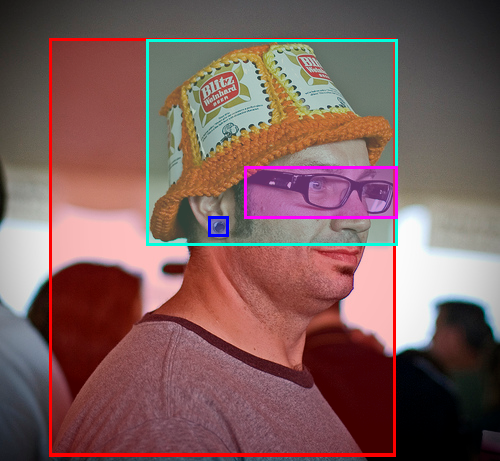
\includegraphics[height=3.0in]{Images/example_hat.png} \vspace{-3mm}&
      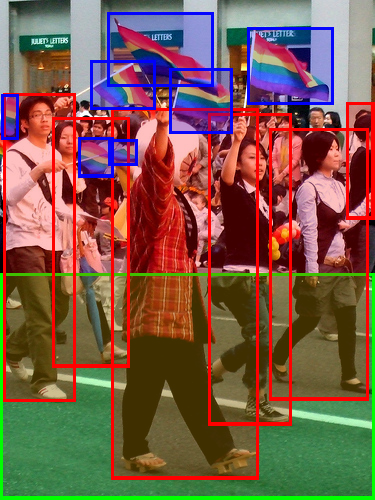
\includegraphics[height=3.0in]{Images/example_parade.png}\\
      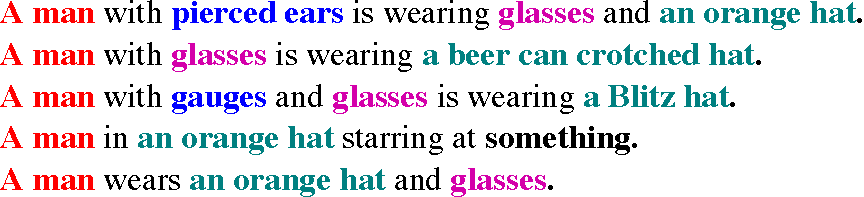
\includegraphics[valign = T,width=.4\columnwidth]{Images/example_hat_text.pdf}&
      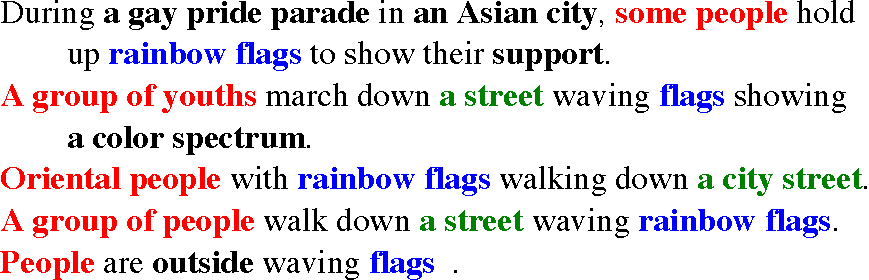
\includegraphics[valign = T,width=.4\columnwidth]{Images/example_parade_text.pdf}
  \end{tabular}
\caption{Voorbeelden van Flickr30k Entities annotaties. De kleur van de frases is overeenkomstig de kleur van de bounding boxes op de afbeelding.}
\label{fig:entities}
\end{figure}

\begin{figure}
    \centering
    \subfloat{
        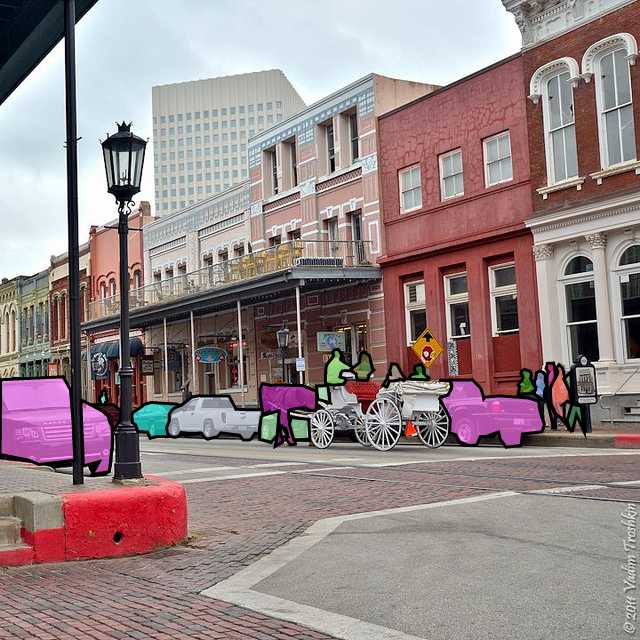
\includegraphics[width=0.47\linewidth]{Images/coco_example1.png}}\hfill
    \subfloat{
        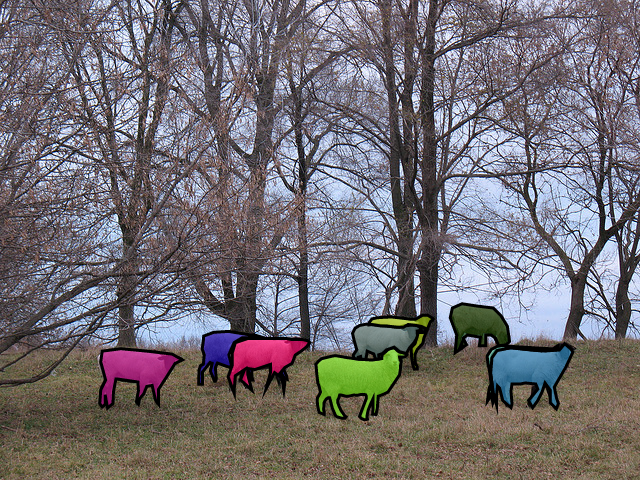
\includegraphics[width=0.47\linewidth]{Images/coco_example2.png}}
    \caption{Voorbeelden van geannoteerde afbeeldingen uit MS COCO dataset. Elk gekleurd object behoort tot \'e\'en van de objectcategorie\"en gedefinieerd door de makers.}
    \label{fig:cocoexamples}
\end{figure}



\subsection{Gebruik}
\label{sub:Gebruik}
Deze dataset bevat zeer veel extra informatie verspreid over een grote hoeveelheid references. Een probleem dat zich voordoet is dat sommige van de bounding boxes zo klein zijn dat er amper informatie uit te halen is. Daarom is er een reductie uitgevoerd van de dataset alvorens over te gaan tot het verwerken van de data. 

De dataset is beschikbaar als tekstbestanden die weergeven welke bounding boxes op welke afbeelding te zien zijn, en met welke delen van de beschrijving elke box overeenkomt. Er zijn een aantal boxes die wel zijn opgenomen in de dataset, maar geen overeenkomstige frase hebben. Voor ons doel zijn deze boxes van mindere waarde, dus ze maken geen deel uit van de dataset die wij hebben aangewend. 

Om de data bruikbaar te maken voor verwerking zijn de tekstbestanden uitgelezen, en zijn alle bounding boxes opgeslagen als aparte afbeelding. Op basis van die afbeeldingen berekent VGGNet een vectorrepresentatie. De overeenkomstige frasen zijn omgezet naar een tf-idf gewogen vectorweergave. 

Op basis van de CCA-uitbreiding beschreven in sectie \ref{sub:stackedcca} berekenen we een geaugmenteerde versie van de afbeeldingen uit de Flickr30k dataset. De extra informatie uit de overeenkomsten tussen bounding boxes en frasen zit vervat in een eerste gemeenschappelijke CCA ruimte. Op basis van \todo{ref naar SAE paper} berekenen we een representatie van de trainingsafbeeldingen, waarin ook de informatie uit de Entities dataset aanwezig is.

Aangezien de Entities dataset enorm groot is, was het nodig om een reductie van het aantal afbeeldingen uit te voeren. Deze reductie gebeurt op basis van de grootte van de bounding box. Een deel van de bounding boxes zijn slechts enkele pixels hoog of breed, waardoor er amper informatie kan worden uit gehaald. Deze bounding boxes worden dus uit de dataset verwijderd. De limiet van zichtbaarheid en informatief zijn van een afbeelding staat ter discussie, maar wij hebben gekozen om alles kleiner dan 64 bij 64 pixels te verwijderen, wat resulteerde in 190,000 bounding boxes en corresponderende frases die we konden gebruiken. 

Het berekenen van de CCA mapping tussen de bounding boxes en de frasen uit de Entities dataset verliep zonder problemen. De berekening van de augmentatie was ook probleemloos, maar tijdens het berekenen van de CCA mapping tussen de augmentaties van de Flickr30k foto's en hun beschrijvingen zijn we tot de conclusie gekomen dat het qua tijdsbestek onhaalbaar was om deze mapping te gebruiken in onze experimenten. 


\section{Toevoeging van LDA topicverdeling aan RNN}
De eerder berekende topicverdelingen kunnen dienen als extra semantische informatie om de generatie in de juiste richting te sturen. Het integreren van de topicverdeling $L$ in het RNN gebeurt volgens formule \eqref{eq:rnnldaonce} die het tweede deel van \eqref{eq:rnn} vervangt.

\begin{equation}
    h_t = f(W_{hx} x_{t} + W_{hh} h_{t-1} + b_h + \mathbbm{1}{(t=1)} \odot b_v +\mathbbm{1}{(t=1)} \odot W_lL
    \label{eq:rnnldaonce}
\end{equation}

Er kan ook gekozen worden om de topicverdeling elke stap toe te voegen, wat leidt tot formule \eqref{eq:rnnldaall}. Het lijkt ons interessant om te experimenteren met het al dan niet altijd toevoegen van de topic informatie. Dit kan, in tegenstelling tot het steeds toevoegen van de afbeelding, een verbetering betekenen. De informatie uit de topicverdeling is afgeleid van de afbeelding, maar bevat informatie van een lagere dimensionaliteit. Het herhaaldelijk meegeven van de topic vector zorgt dat het netwerk elke stap de semantische informatie binnenkrijgt.


\begin{equation}
    h_t = f(W_{hx} x_{t} + W_{hh} h_{t-1} + b_h + \mathbbm{1}{(t=1)} \odot b_v + W_lL
    \label{eq:rnnldaall}
\end{equation}



\section{Canonical Correlation Analysis}
Het toevoegen van extra semantische informatie kan gebeuren op verschillende manieren. Een eerste optie is LDA, zoals eerder beschreven. Er kan echter ook gebruik gemaakt worden van CCA. Waar LDA focust op het blootleggen van verbanden tussen de woorden uit de captions, berekent CCA een ruimte die tussen de afbeelding en de zin ligt.

Het berekenen van deze tussenliggende ruimte gebeurt in twee stappen. Met behulp van het eerder vernoemde VGGNet berekenen we de afbeeldingsvectoren voor de traininggset. De bijhorende zinnen worden voorgesteld door een tf-idf gewogen vector, zoals eerder beschreven. Belangrijk is dat alle zinnen apart worden beschouwd. Waar bij LDA de vij zinnen per afbeelding worden gereduceerd tot \'e\'en zin, blijven ze hier apart. Dit om ervoor te zorgen dat de mapping rekening houdt met de verschillende zinnen. Meer concreet houdt dit in dat elke foto maximaal gecorreleerd dient te zijn met vijf verschillende zinnen uit de trainingsset.

Een deel van de rijkdom van de dataset gaat verloren als er gebruikt wordt gemaakt van een aaneensluiting van de verschillende zinnen. Bij LDA doet dit probleem zich niet voor, en is het zelfs beter om de zinnen bij elkaar te voegen, aangezien de topicverdeling per afbeelding wordt beoogd, en niet per zin. Synoniemen en afgeleiden worden beschouwd als deel van hetzelfde document, juist door de aaneensluiting van de zinnen.

Na het berekenen van de representaties van afbeeldingen en zinnen worden de correlatiecomponenten berekend. Dit gebeurt met de \texttt{MATLAB}-implementatie van het canonical correlation algoritme. Het resultaat bestaat uit twee projectiematrices, die dienen om afbeeldings- en bescrhijvingsvectoren te projecteren op de tussenliggende ruimte die de correlatie maximaliseert. Voor onze experimenten maken we enkel gebruik van de projectie voor afbeeldingen, aangezien jia \todo{REF REF REF} aantoont dat de beste resultaten bereikt worden met het gebruik van enkel de afbeeldingsprojectie.

\section{gLSTM}
\subsection{Guided LSTM}
Guided Long Short Term Memory (gLSTM) is een recente uitbreiding van het LSTM model ge\"introduceerd door Jia et al. \todo{ref} In dit model extraheren ze eerst semantische informatie van elke afbeelding. Deze informatie dient dan als extra input of "gids" voor het LSTM-blok.

Na het bestuderen van bestaande LSTM-modellen ontdekten de auteurs dat de gegenereerde zinnen "semantische drift" vertonen. Dit wil zeggen dat naarmate de zin evolueert, de betekenis van volgende woorden steeds minder met de input-afbeelding te maken heeft. Ze vermoeden dat dit komt door twee tegenwerkende krachten. Enerzijds moet de zin de afbeelding beschrijven, anderzijds moet de zin passen in het taalmodel. Om die reden introduceren ze een semantische gids, die ervoor moet zorgen dat het model na enkele woorden op het juiste pad blijft. Dit gebeurt door aan woorden die semantisch verbonden zijn aan de afbeelding een positieve bias te geven.

Ze gebruiken vier verschillende semantische gidsen in hun experimenten. Als eerste model gebruiken ze een "retrieval-based" gids. Hierbij zoeken ze eerst naar zinnen die gerelateerd zijn aan de afbeelding. Vervolgens verzamelen ze daaruit de zinnen met de hoogste rang. Deze zinnen vormen dan de extra input.
Als tweede model leren ze eerst een CCA-model. Vervolgens nemen de auteurs de projectie van de afbeeldingsrepresentatie in de gemeenschappelijke ruimte. Daarna worden de dichtstbijzijnde geprojecteerde zinnen gezocht op basis van cosinusgelijkheid. Ook hier vormen de hoogst scorende zinnen de extra input.
Een derde model gebruikt de CCA-projectie van de afbeelding in de gemeenschappelijke ruimte rechtstreeks als gids.
Als laatste model gebruiken ze de afbeeldingsrepresentatie zelf als gids.

Om dit te implementeren starten ze net als in deze masterproef van de LSTM-implementatie van Karpathy. Ze defin\"ieren de geheugencellen en poorten zoals in de volgende formules. Hierbij zijn de rode delen toevoegingen ten opzichte van Vinyals\todo{ref} \todo{misschien referentie naar deze formules in theorie?}:

%
\begin{eqnarray}
\vspace{-3mm}
\label{glstm-memory-start}
i_l' & = & \sigma (W_{ix} x_l + W_{im} m_{l-1} \color{red}{+ W_{iq} g}) \label{glstm-input} \\
f_l' & = & \sigma (W_{fx} x_l + W_{fm} m_{l-1} \color{red}{+ W_{fq} g}) \\
o_l' & = & \sigma (W_{ox} x_l + W_{om} m_{l-1} \color{red}{+ W_{oq} g}) \\
c_l' & = & f_l' \odot c_{l-1}' + i_l' \odot h(W_{cx} x_l + \nonumber \\
&   & + W_{cm} m_{l-1} \color{red}{+ W_{cq} g}) \\
m_l & = & o_l' \odot c_l'
\label{glstm-memory}
\vspace{-3mm}
\end{eqnarray}

Hierbij is $g$ de vectorvoorstelling van de semantische informatie. De gids is onafhankelijk van de tijdstap en werkt dus globaal voor elke afbeelding. Figuur \ref{fig:glstm} geeft een visuele voorstelling van de gLSTM-blok.

\begin{figure}[tb][h]
	\centering
	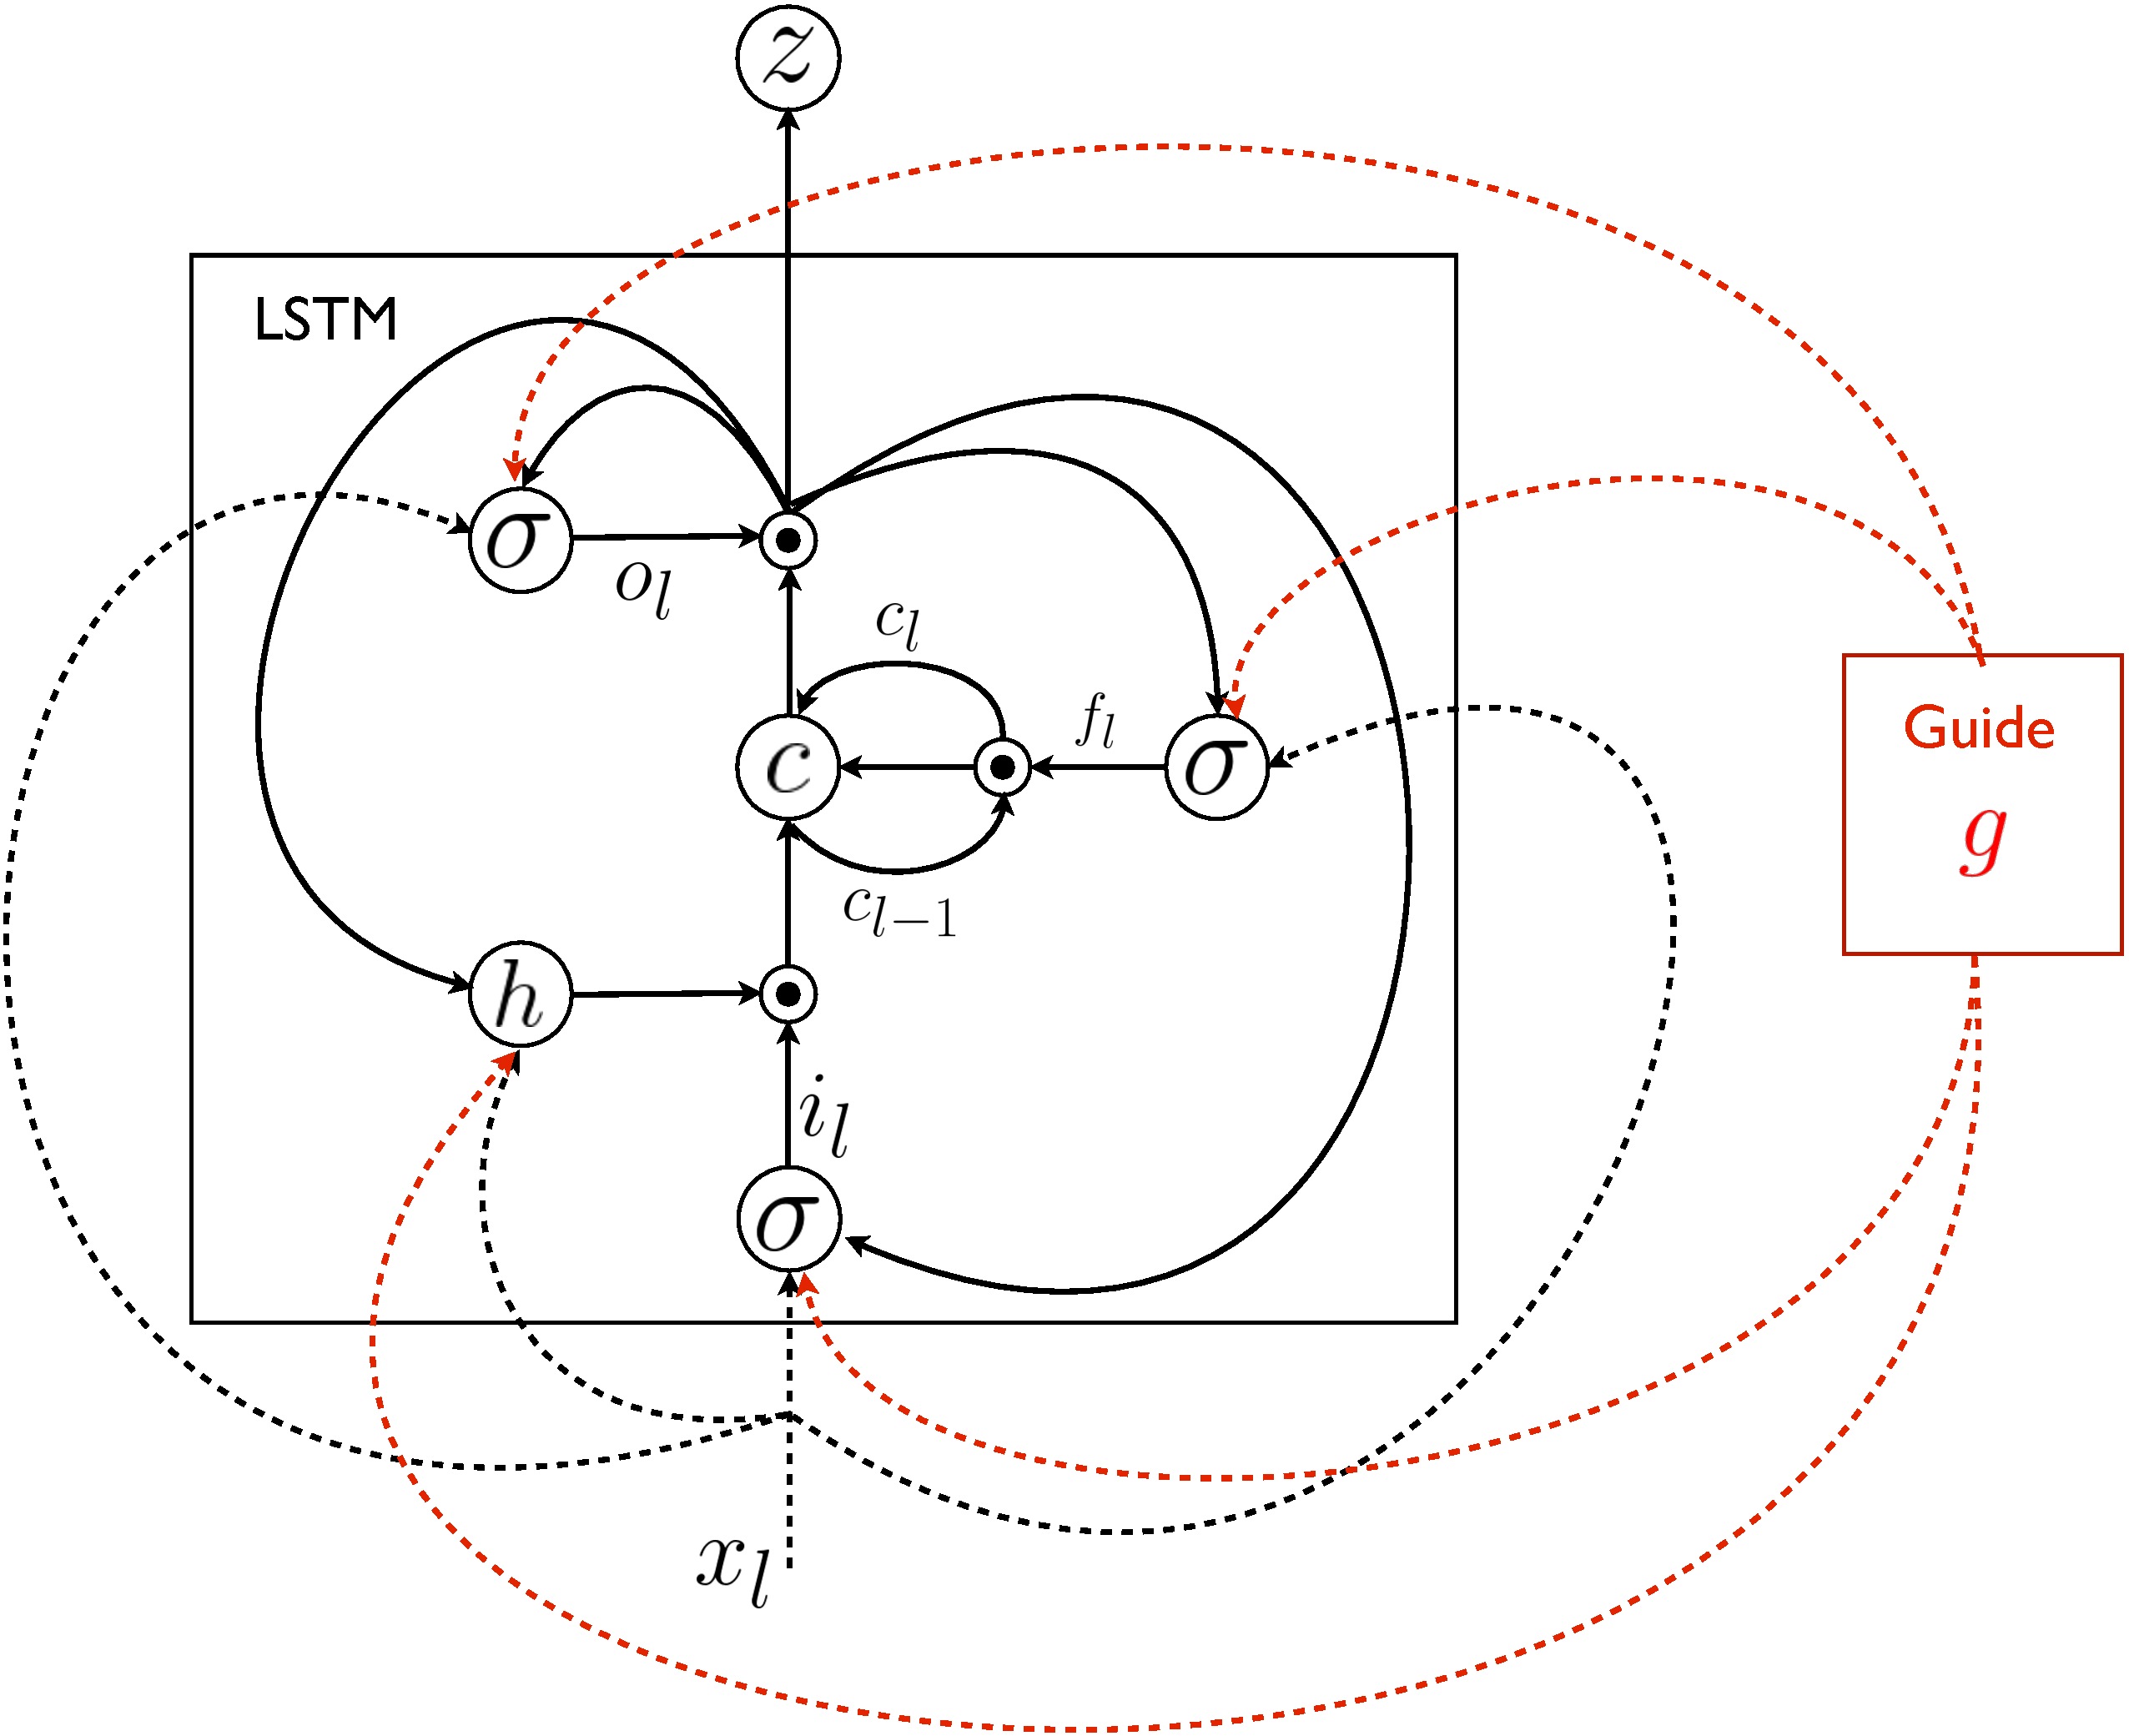
\includegraphics[width=\linewidth]{Images/glstm.pdf}
	\caption{LSTM-blok in het zwart. Uitbreidingen van gLSTM in het rood.}
	\label{fig:glstm}
\end{figure}

Jia et al. bekomen zeer goede resultaten. De eerste drie gidsen zorgen voor verbetering op hun baseline. Enkel de afbeelding als gids zorgt voor verslechtering. De rechtstreekse CCA-projectie presteert het beste.

\subsection{gLSTM met LDA en CCA}
Net als Jia implementeren we de gLSTM als een uitbreiding van LSTM overeenstemmend met formules \ref{glstm-memory-start}-\ref{glstm-memory}.
Om te kunnen vergelijken met hun paper kan onze implementatie ook de CCA-projectie als gids gebruiken.
Daarnaast veronderstellen we dat LDA een goede bron van semantische informatie is. Het bevat immers een verdeling van de onderwerpen die aanwezig zijn in de afbeelding. Daarom kan LDA ook als gids worden gekozen.
We maken dus twee modellen zodat het mogelijk is om na te gaan of LDA een betere gids is dan CCA in onze configuratie van de gLSTM.

\section{Normalisatie van beam search}
Naast het introduceren van gLSTM's breiden Jia et al. \todo{ref} de implementatie van Karpathy nog op een tweede manier uit. Na evaluatie van bestaande modellen leidden ze af dat het gebruikte beam-search algoritme een voorkeur heeft voor kortere zinnen. Beam-search neemt de som van de log-likelihood van individuele woorden als criterium. Aangezien deze waarde voor elk woord negatief is, gaat het algoritme sneller kiezen om te stoppen. Om dit fenomeen tegen te gaan introduceren ze de genormaliseerde log-likelihood van elk woord als criterium.

\begin{equation}
p = \frac{1}{\Omega(\ell)}\sum_{l=1}^{\ell} \log p(s_l | x, s_{1:l}, \theta)
\label{eq:log-sentence-norm}
\end{equation}

In de paper bestuderen ze meerdere functies voor $\Omega$. Wij implementeren de twee meest performante:
Enerzijds de Gaussiaanse functie $\Omega(\ell) \sim \mathcal{N}(\mu, \sigma)$, waar $\mu$ en $\sigma$ respectievelijk het gemiddelde en de standaardafwijking zijn van de lengtes van de zinnen in het trainingscorpus. Hierdoor moeten gegenereerde zinnen gelijkaardige lengtes hebben aan deze uit het corpus.
Anderzijds de min-hinge normalisatie. Met deze methode is de normalisatiefactor gelijk aan de gemiddelde lengte van het trainingscorpus als de zin langer is dan dit gemiddelde. Indien de zin korter is, is de factor gelijk aan de lengte van de zin. Dit komt overeen met de functie $\Omega(\ell)=\min\{\ell, \mu\}$.
